\documentclass[12pt]{article}
\usepackage[margin=1in]{geometry}
\usepackage[all]{xy}
\usepackage{tcolorbox}
\setcounter{section}{1}
\usepackage{dblfloatfix}
\usepackage{amsmath,amsthm,amssymb,color,latexsym}
\usepackage{geometry}        
\usepackage{graphicx}
\geometry{letterpaper}    
\usepackage{graphicx}

\def\bQ{\textbf{Q}}
\def\Err{\text{Err}}
\def\err{\text{err}}

\def\var{\text{Var}}
\def\bx{\textbf{x}}
\def\eps{\varepsilon}
\def\bz{\textbf{z}}
\def\bX{\textbf{X}}
\def\Trace{\text{trace}}
\def\RSS{\text{RSS}}
\def\Cov{\text{Cov}}

\def\by{\textbf{y}}
\def\br{\textbf{r}}

\def\bV{\textbf{V}}
\def\bI{\textbf{I}}
\def\bR{\textbf{R}}
\def\bQ{\textbf{Q}}
\def\bS{\textbf{S}}
\def\bq{\textbf{q}}
\def\bOne{\textbf{1}}

\def\bU{\textbf{U}}
\def\bD{\textbf{D}}
\def\bV{\textbf{V}}
\def\bZ{\textbf{Z}}
\def\bGamma{\mathbf{\Gamma}}

\def\E{\text{E}}
\def\bY{\textbf{Y}}

\newtheorem{exercise}{Exercise}[section]
\tcolorboxenvironment{exercise}{
colframe=gray, before skip=10pt,after skip=10pt }


\newenvironment{solution}[1][\it{Solution}]{\textbf{#1. } }{\vspace{.5cm}}


\begin{document}
\begin{center}
\noindent  \textbf{\Large Elements of Statistical Learning Solutions}
\vspace{.2cm}

\noindent 	Daniel Mitsutani
\end{center}
\newpage


\section{Overview of Supervised Learning}
\hrulefill
\vspace{.6cm}
\begin{exercise}
    Derive equation (2.24).
\end{exercise}
\begin{solution}
    A ball of radius $r$ has volume $r^p \, \text{Vol} \,B(1)$, where $B(1)$ is the unit ball. Hence the probability that a given point lies inside it is $r^p$. The probability that a given point lies outside it is $1-r^p$; the probability that all points lie outside it is $(1-r^p)^N$. The median smallest distance $d(p,N)$ is the radius $r$ such that the probability above is $1/2$. Solving for $r$ gives
    $$d(p,N) = \left(1-\frac{1}{2^{1/N}}\right)^{1/p}$$
\end{solution}

\begin{exercise}Compare the classification performance of linear regression and $k$–
nearest neighbor classification on the zipcode data. In particular, consider
only the 2’s and 3’s, and $k = 1, 3, 5, 7$ and $15$. Show both the training and
test error for each choice. The zipcode data are available from the book
website www-stat.stanford.edu/ElemStatLearn.
\end{exercise}
\begin{solution}
    The results for different $k$ and linear regression are shown below. 

\begin{figure*}[b!]
\centering
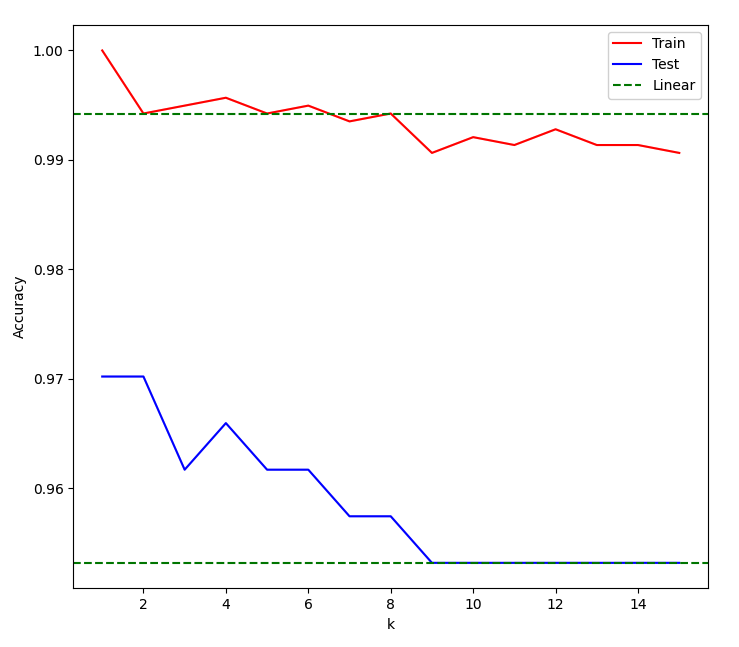
\includegraphics[width = 9.5cm, height = 9.5cm]{fig_2.8.png}
\end{figure*}

\begin{tcolorbox}[width=\linewidth, sharp corners=all, colback=white!95!black]

    \begin{verbatim}
import numpy as np
from sklearn.neighbors import KNeighborsClassifier as KNClassifier
from sklearn.linear_model import LinearRegression
from sklearn.metrics import accuracy_score as accuracy
from matplotlib import pyplot as plt

train_data = np.loadtxt('training_data')
train_df = train_data[np.where
           ((train_data[:, 0] == 2) | (train_data[:, 0] == 3))]

test_data = np.loadtxt('test_data')
test_df = test_data[np.where
          ((test_data[:, 0] == 2) | (test_data[:, 0] == 3))]

X_train, X_test = train_df[:, 1:], test_df[:, 1:]
y_train, y_test = train_df[:, 0].reshape(-1), test_df[:, 0].reshape(-1)

k_list = range(1,16)
classifiers = []
for k in k_list:
    classifier = KNClassifier(k, n_jobs = -1)
    classifier.fit(X_train, y_train)
    classifiers.append(classifier)

accs_train = []
accs_test = []
for i in range(len(k_list)):
    y_train_predict = classifiers[i].predict(X_train)
    y_test_predict = classifiers[i].predict(X_test)
    accs_train.append(accuracy(y_train_predict, y_train))
    accs_test.append(accuracy(y_test_predict, y_test))

lin_model = LinearRegression()
lin_model.fit(X_train, y_train)
linear_train_acc = accuracy(y_train, lin_model.predict(X_train).round())
linear_test_acc = accuracy(y_test, lin_model.predict(X_test).round())
\end{verbatim}
\end{tcolorbox}
\newpage

\begin{tcolorbox}[width=\linewidth, sharp corners=all, colback=white!95!black]

    \begin{verbatim}
plt.plot(k_list, accs_train, color = 'red', label = 'Train')
plt.plot(k_list, accs_test, color = 'blue', label = 'Test')
plt.axhline(
    linear_train_acc, color = 'green', label = 'Linear', ls = '--')
plt.axhline(linear_test_acc, color = 'green', ls = '--')

plt.xlabel('k')
plt.ylabel('Accuracy')
plt.legend()
plt.show()
\end{verbatim}
\end{tcolorbox}
\end{solution}

\begin{exercise}
    Suppose we have a sample of $N$ pairs $x_i, y_ii$ drawn i.i.d. from the distribution characterized as follows:
    \begin{center}
    $$\begin{aligned}&x_i \sim h(x), \text{ the design density}\\
    &y_i = f(x_i) + \varepsilon_i, \, f \text{ is the regression function}\\
    &\eps_i \sim (0, \sigma^2)\, \text{(mean zero, variance $\sigma^2$)}
    \end{aligned}$$
    \end{center}
    We construct an estimator for $f$ linear in the $y_i$,
$$\hat{f}(x_0) = \sum_{i = 1}^N \ell_i(x_0; \mathcal{X})y_i$$
where the weights $\ell_i(x_0, \mathcal{X})$ do not depend on the $y_i$, but do depend on the
entire training sequence of $x_i$, denoted here by $\mathcal{X}$.
\begin{enumerate}
\item[(a)] Show that linear regression and k-nearest-neighbor regression are members
of this class of estimators. Describe explicitly the weights $\ell_i(x_0, \mathcal{X})$
in each of these cases.
\item[(b)] Decompose the conditional mean-squared error
$$\E_{\mathcal{Y}| \mathcal{X}}[(f(x_0) - \hat{f}(x_0))^2]$$
into a conditional squared bias and a conditional variance component.
Like $\mathcal{X}$, $\mathcal{Y}$ represents the entire training sequence of $y_i$.
\item[(c)] Decompose the (unconditional) mean-squared error
$$\E_{\mathcal{Y}, \mathcal{X}}[(f(x_0) - \hat{f}(x_0))^2]$$
into a squared bias and a variance component.
\item[(d)] Establish a relationship between the squared biases and variances in
the above two cases.
\end{enumerate}
\end{exercise}
\begin{solution}\begin{enumerate}
    \item [(a)]  For linear regression, $\hat{f}(x_0) = x_0^T \beta$, where $\beta = (\bX^T\bX)^{-1}\bX^T y$, so that $$\ell_i(x_0; \mathcal{X}) = x_0^T(\bX^T\bX)^{-1}x_i$$
    For $k$-nearest-neighbors, we may write:
    $$\hat{f}(x_0) = \frac{1}{k}\sum_{x_i \in N_k(x_0)} y_i,$$
    so that:
    $$\ell_i(x_0, \mathcal{X}) = \frac{1}{k} I_{N_k(x_0)}(x_i),$$
    and $I_{N_k(x_0)}$ is the indicator function of the $k$-nearest neighbors of $x_0$.

    \item [(b)]
    $$\begin{aligned}\E_{\mathcal{Y}| \mathcal{X}}[(f(x_0) - \hat{f}(x_0))^2] &= \E_{\mathcal{Y}| \mathcal{X}}[\hat{f}(x_0)^2] -2 f(x_0)\E_{\mathcal{Y}| \mathcal{X}}[\hat{f}(x_0)] + f(x_0)^2 \\
    &= \E_{\mathcal{Y}| \mathcal{X}}[\hat{f}(x_0)^2]- \E_{\mathcal{Y}| \mathcal{X}}[\hat{f}(x_0)]^2\\
    &+ \E_{\mathcal{Y}| \mathcal{X}}[\hat{f}(x_0)]^2 -2 f(x_0)\E_{\mathcal{Y}| \mathcal{X}}[\hat{f}(x_0)] + f(x_0)^2 \\
    &= \var_{\mathcal{Y}|\mathcal{X}}(\hat{f}(x_0)) + (\E_{\mathcal{Y}| \mathcal{X}}[\hat{f}(x_0)]- f(x_0))^2 
    \end{aligned}$$
    The second term is the conditional square bias. 
    \item [(c)] Similarly:
    $$\E_{\mathcal{Y}, \mathcal{X}}[(f(x_0) - \hat{f}(x_0))^2]  = \var_{\mathcal{Y},\mathcal{X}}(\hat{f}(x_0)) + (\E_{\mathcal{Y}, \mathcal{X}}[\hat{f}(x_0)]- f(x_0))^2 $$

    \item [(d)] We now use the linearity assumption. For simplicity, we write $y$ and $L = \ell(x_0, \mathcal{X})$ to be the coresponding vectors, so that $\hat{f}(x_0) = L^T y$. Further, we let $f(\mathcal{X}) = (f(x_1), \dots, f(x_n))$ and $\eps = f(\mathcal{X})-y$. Then
    $$\E_{\mathcal{Y}| \mathcal{X}}[\hat{f}(x_0)]- f(x_0) =  \E_{\mathcal{Y}| \mathcal{X}}[L^T(f(\mathcal{X})+\eps)]- f(x_0) = L^Tf(\mathcal{X})-f(x_0)$$
    and
    $$\var_{\mathcal{Y}|\mathcal{X}}(\hat{f}(x_0)) = \var_{\eps}(L^T\eps) = \, \sigma^2 L^T L $$

    
\end{enumerate}
\end{solution}

\begin{exercise}
    Consider a linear regression model with $p$ parameters, fit by least
squares to a set of training data $(x_1, y_1), . . . , (x_N, y_N)$ drawn at random
from a population. Let $\hat{\beta}$ be the least squares estimate. Suppose we have
some test data $(\tilde{x}_1, \tilde{y}_1), . . . , (\tilde{x}_M, \tilde{y}_M)$ drawn at random from the same population
as the training data. If $R_{tr}(\beta) =\frac{1}{N} \sum_{i=1}^N(y_i - \beta^T x_i)^2$ and $R_{te}(\beta) =\frac{1}{M} \sum_{i=1}^M(\tilde{y}_i - \beta^T \tilde{x}_i)^2$ prove that
$$E[R_{tr}(\hat{\beta})] \leq  E[R_{te}(\hat{\beta})]$$
where the expectations are over all that is random in each expression. [This
exercise was brought to our attention by Ryan Tibshirani, from a homework
assignment given by Andrew Ng.]
\end{exercise}
\begin{solution}
    Note that the terms $(\tilde{y}_i - \hat{\beta}^T \tilde{x}_i)^2$ are i.i.d. in $(\tilde{x}_i, \tilde{y}_i)$ since $\hat{\beta}$ only depends on the training data. Thus, the RHS of the inequality is independent of $M$ and we may set $M = N$. 
    
    For the test data $(\tilde{x}_1, \tilde{y}_1), . . . , (\tilde{x}_N, \tilde{y}_N)$, let $\tilde{\beta}$ be the least squares estimate of $\beta$. By definition $R_{te}(\hat{\beta}) \geq R_{te}(\tilde{\beta})$ so that:
    $$E[R_{te}(\hat{\beta})] \geq E[R_{te}(\tilde{\beta})].$$
    
    On the other hand, since the number of samples and the distribution of the test data and training data are the exact same, $R_{te}(\tilde{\beta})$ is equal in distribution to $R_{tr}(\hat{\beta})$. Thus the RHS of the above inequality is in fact equal to $E[R_{tr}(\hat{\beta})]$, and we are done.
\end{solution}



\newpage
\section{Linear Methods for Regression}
\hrulefill
\vspace{.6cm}


\begin{exercise}
		Show that the $F$ statistic (3.13) for dropping a single coefficient
		from a model is equal to the square of the corresponding $z$-score (3.12).
\end{exercise}
\begin{solution}
	Let $\hat{\by}_0$ and $\hat{\by}_1$ be the estimators of $\by$ with the $j$-th variable removed and the full model, respectively. Then  $\hat{\by}_0$ is the projection of $\by$ onto the span of the $\bx_i$ with $i \neq j$ and $\hat{\by}_1$ is the projection of $\by$ onto the span of the $\bx_i$. By the Pythagorean Theorem:
	$$\RSS_0 = \|\hat{\by}_0 - \by\|^2 = \|\hat{\by}_1 - \by\|^2 + \frac{\langle \by, \bz_j\rangle^2}{\|\bz_j\|^2} = \RSS_1+ \frac{\langle \by, \bz_j\rangle^2}{\|\bz_j\|^2}, $$
	where $\bz_j$ is the residual of $\bx_j$ regressed on the remaining $\bx_i$. 
	
	Further, $\RSS_1 = (N-p_1 -1) \hat{\sigma}^2$ by (3.8) so that:
	$$F = (N - p_1 -1 )\cdot  \frac{\RSS_0-\RSS_1}{\RSS_1} = \frac{\langle \by, \bz_j\rangle^2}{\hat{\sigma}^2\|\bz_j\|^2} = \frac{\hat{\beta_j}^2 \|\bz_j\|^2}{\hat{\sigma}^2},$$
	where we used (3.28). To conclude, recall that:
 $$\var(\hat{\beta}_j) = v_j \sigma^2 = \frac{\sigma^2}{\|z_j\|^2},$$
 and use the definition of the $z$-score.
\end{solution} 

\begin{exercise} Given data on two variables $X$ and $Y$, consider fitting a cubic
polynomial regression model $f(X) = \sum_{j = 0}^3 \beta_j X^j$. In addition to plotting
the fitted curve, you would like a 95\% confidence band about the curve. Consider the following two approaches:
\begin{enumerate}
\item  At each point $x_0$, form a 95\% confidence interval for  the linear function $$a^T \beta = \sum_{j = 0}^3 \beta_j x_0^j$$

\item Form a 95\% confidence set for $\beta$ as in (3.15), which in turn generates
confidence intervals for $f(x_0)$.
\end{enumerate}
How do these approaches differ? Which band is likely to be wider? Conduct
a small simulation experiment to compare the two methods.
\end{exercise} 
\begin{solution}
    For method 1, since $\hat{\beta} \sim N(\beta, (\bX^T\bX)^{-1} \sigma^2)$ then $a^T \hat{\beta} \sim N(a^T\beta, a^T(\bX^T\bX)^{-1}a \sigma^2)$. Hence the 95\% confidence interval for $x_0^T \beta$ is:
    $$x_0^T \hat{\beta} \pm 1.96 \cdot \sigma \sqrt{x_0^T(\bX^T\bX)^{-1}x_0}.$$

    For method 2, the confidence set for $\beta$ is given by:
    $$C_\beta = \{\beta: (\beta-\hat{\beta})^T \bX^T \bX (\beta-\hat{\beta}) \leq \hat{\sigma}^2 {\chi^2(0.95, 4)}\}$$

    Letting $LL^T$ be the Cholesky decomposition of $\bX^T\bX$, any $\beta$ on the boundary of $C_\beta$ is of the form:
    $$\beta = \hat{\beta} + (L^T)^{-1}\delta,$$
    where $\delta$ is a vector on the sphere of radius $\hat{\sigma} \sqrt{\chi^2(0.95, 4)}$. The error on $y$ is then given by $x_0^T (L^T)^{-1} \delta$. If $\delta$ is the most expanded direction (in the SVD) of $(L^T)^{-1}$, this may exceed the error of the former method. We illustrate this in the image above generated from the code that follows.


\begin{figure}
\centering
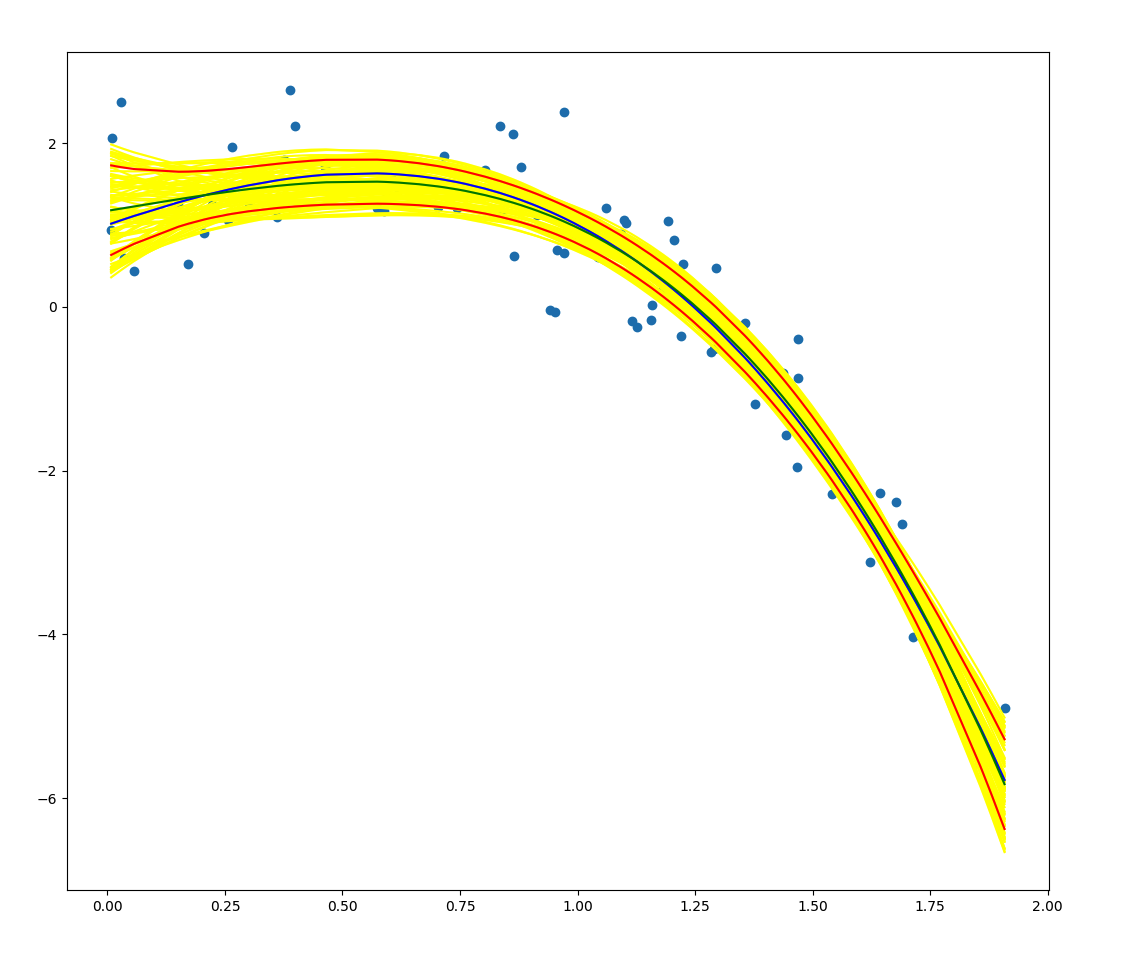
\includegraphics[width = 12cm, height = 11cm]{fig_3.2.png}
\caption{The blue and green lines are the actual and predicted (by OLS) curves for a cubic polynomial.
The yellow shaded region are in fact the graphs of 100 $\beta's$ obtained by method 2 for different $\delta$ uniformly distributed on the sphere of appropriate radius. The red lines are the error bands for method 1. }

\end{figure}

\begin{tcolorbox}[width=\linewidth, sharp corners=all, colback=white!95!black]

    \begin{verbatim}
import numpy as np
from matplotlib import pyplot as plt
from scipy.stats import chi2

x_min = 0
x_max = 2
n = 100
sigma = 0.7
p = 0.95
df = 4
num = 100

f = lambda x: 1 + 2 * x - x ** 2 - x ** 3
f_vec = np.vectorize(f)

def make_X(n, x_min, x_max):
    x0 = np.ones(n)
    x1 = np.sort((x_max-x_min) * np.random.random(n) + x_min)
    x2 = np.square(x1)
    x3 = np.power(x1, 3)
    return np.column_stack((x0, x1, x2, x3))

X = make_X(n, x_min, x_max)

y_actual = f_vec(X[: , 1].T)
y_observed = y_actual + sigma*np.random.normal(0, sigma, n)
y_var = np.sqrt(np.diag(X @ np.linalg.inv(X.T @ X) @ X.T))

beta_ols = np.linalg.inv(X.T @ X) @ X.T @ y_observed
y_predict = X @ beta_ols

y_max_1 = y_predict + 1.96 * sigma * y_var
y_min_1 = y_predict - 1.96 * sigma * y_var

L = np.linalg.cholesky(X.T @ X)
U = L.T
U_inv = np.linalg.inv(U)
for i in range(num):
    delta = np.random.normal(0,1,4)
    delta = delta * sigma * np.sqrt(chi2.ppf(p, df))
            /(np.linalg.norm(delta, ord = 2))
    delta = U_inv @ delta
    beta_sim = beta_ols + delta
    plt.plot(X[:, 1], X @ beta_sim, color = 'yellow')
\end{verbatim}
\end{tcolorbox}
\begin{tcolorbox}[width=\linewidth, sharp corners=all, colback=white!95!black]

    \begin{verbatim}
plt.scatter(X[:, 1], y_observed)
plt.plot(X[:, 1], y_actual, color = 'blue')
plt.plot(X[:, 1], y_predict, color = 'green')
plt.plot(X[:, 1], y_max_1, color = 'red')
plt.plot(X[:, 1], y_min_1, color = 'red')
plt.show()
\end{verbatim}
\end{tcolorbox}

\end{solution}

\begin{exercise}Gauss–Markov theorem:
\begin{enumerate}
\item[(a)] Prove the Gauss–Markov theorem: the least squares estimate of a
parameter $a^T \beta$ has variance no bigger than that of any other linear
unbiased estimate of $a^T \beta$ (Section 3.2.2).
\item[(b)] The matrix inequality $B \prec A$ holds if $B-A$ is positive semidefinite. Show that if $\hat{\bV}$ is the variance-covariance matrix of the least squares estimate of $\beta$ and $\tilde{\bV}$ is the variance-covariance matrix of any other
linear unbiased estimate, then $\hat{\bV} \prec \tilde{\bV}$.
\end{enumerate}
\end{exercise}

\begin{solution}
    \begin{enumerate}
    \item [(a)] Write $c^T = a^T (\bX^T \bX)^{-1} \bX^T + \Delta^T$. Then:
    $$\E(c^T y) = \E((a^T (\bX^T \bX)^{-1} \bX^T + \Delta^T)y) = a^T \beta + \E(\Delta^T X \beta),$$
    and since $c^T y$ is unbiased we have $\Delta^T X = 0$.

    For simplicity, let $a^T (\bX^T \bX)^{-1} = M$. Now we compute the variance:
    $$\begin{aligned} \var(c^Ty) &= \E(y^T c c^T y) - (a^T\beta)^2 \\
    &= \E(y^T (M\bX^T + \Delta^T)^T (M\bX^T + \Delta^T) y) - (a^T\beta)^2 \\
    &= \E(y^T(M\bX^T)^T(M\bX^T)y) - (a^T\beta)^2 + \E(y^T\Delta\Delta^Ty) \\
    &= \var_{OLS} + \E((\Delta^T y)^2),
    \end{aligned}$$
    where on the third line we used $\Delta^T X  = 0$. Since $\E((\Delta^T y)^2) \geq 0$, this concludes the proof.

    \item [(b)] The proof is the same but in matrix form.
    \end{enumerate}
\end{solution}

\begin{exercise} Show how the vector of least squares coefficients can be obtained from a single pass of the Gram-Schmidt procedure (Algorithm 3.1). Represent your solution in terms of the QR decomposition of $\bX$.
\end{exercise}
\begin{solution}
    By (3.32), $\hat{\beta} = \bR^{-1}\bQ^T \by$. Since $\bQ = \bZ \bD^{-1}$, $\bQ$ can be computed as one obtains $\bz_i$ in the Gram-Schmidt algorithm by entering the normalized $\bz_i$. Similarly, $\bR = \bD \bGamma$, is immediately found as the entries of $\hat{\gamma}_{kj}$ with the normalized $\bz_i$. Since $\bR$ is upper triangular, it can be inverted quickly.
\end{solution}

\begin{exercise} Consider the ridge regression problem (3.41). Show that this problem is equivalent to the problem
$$\hat{\beta}^c = \arg \min_{\beta^c} \left\{ \sum_{i = 1}^N [y_i - \beta_0^c - \sum_{j = 1}^p (x_{ij} - \bar{x}_j)\beta_j^c]^2 + \lambda \sum_{j =1}^p {\beta_j^c}^2 \right\}$$
Give the correspondence between $\beta^c$ and the original $\beta$ in (3.41). Characterize tthe solution to this modified criteriion. Show that a similar result holds for the lasso.
\end{exercise}
\begin{solution} Letting $\beta_0 = \beta_0^c - \sum_{j=1}^p \bar{x}_j \beta_j^c$, and $\beta_i = \beta_i^c$ for $i \neq 0$, the problem above becomes the usual lasso
$$\hat{\beta} = \arg \min_{\beta} \left\{ \sum_{i = 1}^N [y_i - \beta_0 - \sum_{j = 1}^p x_{ij}\beta_j]^2 + \lambda \sum_{j =1}^p {\beta_j}^2 \right\}$$
From the relations between $\beta$ and $\beta^c$, we see that the slope coefficients for the centered problem are the same, whereas the intercept $\beta^c_0 = \beta_0 + \bar{\bx}^T \beta$ is the predicted value (by the usual lasso) at the mean of the data. The analysis for ridge is identical, since it only changes the penalty term.
\end{solution}
\begin{exercise}
    Show that the ridge regression estimate is the mean (and mode) of the posterior distribution, under a Gaussian prior $\beta \sim N(0, \tau^2 \bI)$, and Gaussian sampling model $\by \sim N(\bX \beta, \sigma^2 \bI)$. Find the relationship between the regularization parameter $\lambda$ in the ridge formula, and the variances $\tau$ and $\sigma^2$.
\end{exercise}
\begin{solution}
    By Bayes' formula:
    $$f(\beta | \by, \bX) \propto f(\by, \bX | \beta) f(\beta) \propto f(\by | \bX, \beta) f(\beta),$$
    since $f(\bX)$ does not depend on $\beta$.  Thus:
    $$\begin{aligned}f(\beta | \by, \bX) &\propto \exp\left(-\frac{(\by-\bX\beta)^T(\by-\bX\beta)}{2\sigma^2} - \frac{1}{2\tau^2}\beta^T \beta\right)\\
    &\propto \exp\left(\frac{-1}{2\sigma^2}\left(-\beta^T\left(\bX^T\bX + \frac{\sigma^2}{\tau^2} \bI\right)\beta + \by^T\bX\beta + \beta^T \bX^T \by\right)\right)
    \end{aligned}$$
    
    Recall in general that a multivariate Gaussian in $\beta$ with mean $\mu$ and covariance matrix $\Sigma$ has pdf proportional to
    $$\exp\left(-\frac{(\beta-\mu)^T\Sigma^{-1}(\beta-\mu)}{2}\right) \propto \exp\left(-\frac{\beta^T\Sigma^{-1}\beta +\beta^T\Sigma^{-1}\mu + \mu^T(\Sigma^{-1})^T\beta}{2}\right)$$
    Comparing the two, we see that the pdf $f(\beta | \by, \bX)$ is indeed Gaussian with $$\Sigma^{-1} = \frac{1}{\sigma^2}\left(\bX^T\bX + \frac{\sigma^2}{\tau^2} \bI\right),$$
    and moreover we see that $\bX^T\by = \sigma^2 \Sigma^{-1}\mu$ by comparing the third term in $f(\beta | \by, \bX)$ with the second term in the general Gaussian pdf. Solving for $\mu$ and plugging $\Sigma^{-1}$ found as above gives:
    $$\mu = \left(\bX^T\bX + \frac{\sigma^2}{\tau^2} \bI\right)^{-1}\bX^T\by,$$
    which is precisely $\beta^{ridge}$ with $\lambda = \sigma^2/\tau^2$, as desired.
\end{solution}

\begin{exercise}
Consider the decomposition of the uncentered $N \times (p+1)$ matrix $\bX$ whose first column is all ones), and the SVD of the $N \times p$ centered matrix $\tilde{\bX}$. Show that $\bQ_2$ and $\bU$ span the same subspace, where 
$\bQ_2$ is the sub-matrix of $\bQ$ with the first column removed. Under what circumstances will they be the same, up to sign flips?
\end{exercise}
\begin{solution}
Recall that $\bQ = \bZ \bD^{-1}$, where $\bZ$ is the vector of residuals obtained in the Gram-Schmidt algorithm. Hence, $\bq_0$ is a scalar multiple of $\bOne$, since $\bz_0 = \bOne$. Since $\bQ$ is orthogonal, the span of $\bQ_2$ is equal to span$(\bQ) \cap \bOne^\perp$, where $\perp$ denotes orthogonal complement. Moreover span$(\bQ) = $ span$(\bX)$, since $\bR$ is invertible. Hence span$(\bQ_2) = $ span$(\bX) \cap \bOne^\perp$.

Clearly also span$(\bU) = $ span$(\tilde{\bX})$, since again $\bD\bV$ is invertible. But note that $\tilde{\bx}_i$ is simply the projection of $\bx_i$ onto $\bOne^\perp$, since $\tilde{\bx}_i = \bx_i - \bar{x}_i \bOne$, where $\bar{x}_i  = (1/N) \bx_i^T \bOne$. Hence span$(\bU) = $ span$(\tilde{\bX}) = $ span$(\bX) \cap \bOne^\perp$ and the first part of the exercise is complete.

For these to agree, we need $\bD \bV = \bR$, i.e., an orthogonal matrix is equal to an upper-triangular one. Thus both have to be the identity (up to sign flips) and $\bX = \bQ$ (up to sign flips), i.e. the feature input vectors $\bx_i$ must have been orthogonal to begin with.


\end{solution}

\begin{exercise}
    Forward stepwise regression. Suppose we have the QR decomposition for the $N \times p$ matrix $\bX_1$ in a multiple regression problem with response $\by$, and we have an additional $p-q$ predictors in the matrix 
$\bX_2$. Denote the current residual by $\br$. We wish to establish which one of these additional variables will reduce the residual sum-of-squares the most when included with those in 
$\bX_1$. Describe an efficient procedure for doing this.
\end{exercise}
\begin{solution}
Let $\by_0$ be the current predictor of $\by$, i.e., $\by = \by_0 + \br$. Then $\by_0$ is the orthogonal projection of $\by$ onto the column span of $\bQ$. If we add a new column $\bx_{p+1}$, the new residual will be given by the projection of $\bR$ we on the span columns of $\bQ$ and $\bx$.  Letting $\bz_{p+1}= \bx_{p+1} - \sum_{i=1}^p \langle \bx_{p+1}, \bq_i \rangle \bq_i$ be the orthogonal component of $\bx_{p+1}$ relative to the column span of $\bQ$, we can write the residue $\br$ as 
$$\br = \br' + \frac{\langle \br, \bz_{p+1}\rangle}{\langle \bz_{p+1}, \bz_{p+1}\rangle} \bz_{p+1},$$
where $\br'$ will be the new residues after adding $\bx_{p+1}$. Hence the difference in RSS is given by $|\langle \br, \bz_{p+1} \rangle |/\|\bz_{p+1}\|$. We can perform this procedure for all columns of $\bX_2$ and find the largest value. 

Note that this also allows us to update the QR decomposition for the next step as well via $\bq_{p+1} = \bz_{p+1}/\|\bz_{p+1}\|$.
\end{solution}

\begin{exercise} Backward stepwise regression. Suppose we have the multiple regression fit of 
$\bX$ on $\by$ , along with the standard errors and $Z$-scores as in Table 3.2. We wish to establish which variable, when dropped, will increase residual sum-of-squares the least. How would you do this?
\end{exercise}
\begin{solution}
    By Exercise 3.1, the residual sum of squares difference ($F$-score) is proportional to the $Z$-score when dropping a single variable. Hence we simply pick the variable with smallest $Z$-score to drop.
\end{solution}

\begin{exercise} Show that the ridge regression estimates can be obtained by ordinary least squares regression on an augmented data set. We augment
the centered matrix $\bX$ with $p$ additional rows $\sqrt{r\mathbf{I}}$, and augment y with p
zeros. By introducing artificial data having response value zero, the fitting
procedure is forced to shrink the coefficients toward zero. This is related to
the idea of hints due to Abu-Mostafa (1995), where model constraints are
implemented by adding artificial data examples that satisfy them.
\end{exercise}

\begin{solution}
    The ordinary least squares regression solves:
    $$\hat{\beta}^{OLS} = \arg\min_{\beta} \|\by - \bX \beta\|^2$$
    For the augmented matrix $\bX$ and the augmented $\by$, by the Pythagorean theorem this is simply:
    $$\hat{\beta}^{ridge} = \arg\min_{\beta} \|\by - \bX \beta\|^2 + \|\mathbf{0} -\sqrt{\lambda} \beta\|^2 = \arg\min_{\beta} \|\by - \bX \beta\|^2 + \lambda \|\beta\|^2,$$
    which is the Ridge regression estimator.

\end{solution}

\begin{exercise}
    Suppose for a given $t$ in (3.51) the fitted lasso coefficient for the variable $X_j$ is $\hat{\beta}_j = a$. Suppose we augment our set of variables with an identical copy $X^*_j = X_j$. Characterize the effect of this exact collinearity by describing the set of solutions for $\hat{\beta}_j$ and $\hat{\beta}_j^*$ using the same value of $t$.
\end{exercise}
\begin{solution}
    We will consider adding a copy of the last column $\bx_p$. The constrained form of lasso regression is 
    $$\hat{\beta}^{lasso} = \arg \min_\beta \sum_{i = 1}^N \left(y_i - \beta_0 - \sum_{j=1}^p x_{ij}\beta_j\right)^2 = \arg \min_\beta \sum_{i = 1}^N \left(y_i - \beta_0 - \sum_{j=1}^{p-1} x_{ij}\beta_j - x_{ip}\beta_p\right)^2.$$
    subject to $\sum_{j = 1}^p |\beta_j| \leq t$.
    By augmenting with a copy as explained, we add a column $x_{i (p+1)} = x_{ip}$ with coefficient $\beta_{p+1}$, so the new optimization problem is:
    $$\hat{\beta}^{lasso} = \arg \min_\beta \sum_{i = 1}^N \left(y_i - \beta_0 - \sum_{j=1}^{p-1} x_{ij}\beta_j - x_{ip}(\beta_p+\beta_{p+1})\right)^2$$
    subject to $\sum_{j = 1}^{p+1} |\beta_j| \leq t$. Let $\beta_p^0$ be the estimator for $\beta_p$ for the original problem without the copied variable. For the new problem, as long as $\beta_p + \beta_{p+1} = \beta_p^0$ and $|\beta_p| + |\beta_{p+1}| = |\beta_p^0|$ with other coefficients being equal then we have a solution to the new optimization problem which is on the boundary. 

    Therefore adding the copy of a variable creates ambiguity on the coefficients of the copied variable and its copy, i.e., any choice of the form $\beta_p = t\beta_p^0$, $\beta_{p+1} = (1-t)\beta_p^0$ for $t \in [0,1]$ will be a solution to lasso regression. 
\end{solution}

\setcounter{section}{6}
\newpage
\section{Model Assesment and Selection}
\hrulefill
\vspace{.6cm}
\begin{exercise}
    Derive the estimate of in-sample error (7.24). 
\end{exercise}
\begin{solution}
    The estimate (7.24) is obtained by plugging (7.23) into (7.22). It remains to derive (7.23), assuming additive errors $Y = f(X) + \eps$ and a linear model $\hat{Y} = \bS Y$. In what follows since we deal with in-sample errors all expectations are taken over $Y$, i.e., $X$ is assumed to be fixed. Note that
        $$\sum_{i=1}^N \Cov(\hat{y}_i, y_i) = \Trace \, (\Cov (\hat{Y}, Y)),$$
    so that it remains to expand the covariance matrix:
    $$\begin{aligned}\Trace \, (\Cov (\hat{Y}, Y)) &= \Trace\,  (\E[(\hat{Y}- \E(\hat{Y}))(Y- \E[Y])^T])\\
    &= \Trace\,  (\E[(\bS (f(X) + \eps) - \E(\bS (f(X) + \eps)))(f(X)+\eps- \E[f(x)+\eps])^T])\\
    &= \Trace\,  (\E[(\bS (f(X) + \eps) - \E[\bS f(X)])(f(X)+\eps- \E[f(X)])^T])\\
    & =\Trace\,  (\E[(\bS (f(X) + \eps) - \E[\bS f(X)])\eps^T)\\
    &= \Trace\,  (\E[\bS \eps \eps^T]),
    \end{aligned}$$
    since all the terms not involving $\eps$ cancel out and $\E[\eps] = 0$. Using the linearity of expectation:
    $$\Trace\,  (\E[\bS \eps \eps^T]) = \Trace\, (\bS \E[\eps \eps^T])] = \sigma_\eps^2\, \Trace(\bS),$$
    since $\eps$ is assumed to have mean 0 and variance $\sigma_\eps^2 I_N$.
    By definition $d= \Trace(\bS)$, which completes the proof. 
    
\end{solution}

\begin{exercise}
    Consider the in-sample prediction error (7.18) and the training error $\overline{\err}$ in the case of squared-error loss:
    $$\begin{aligned}
        \Err_{in} &= \frac{1}{N} \sum_{i=1}^N E_{Y^0}(Y_i^0 - \hat{f}(x_i))^2 \\
        \overline{err} &= \frac{1}{N} \sum_{i=1}^N (y_i - \hat{f}(x_i))^2
    \end{aligned}$$
    Add and subtract $f(x_i)$ and $E\hat{f}(x_i)$ in each expression and expand. Hence establish that the average optimism in the training error is
    $$\frac{2}{N}\sum_{i=1}^N \Cov\,(\hat{y}_i, y_i),$$
    as given in (7.21).
\end{exercise}
\begin{solution}
    Write $\hat{y_i} = \hat{f}(x_i)$. Adding and subtracting we can group:
    $$Y_i^0 - \hat{f}(x_i) = (Y_i^0-f(x_i)) + (f(x_i) - \E\hat{y}_i) + (\E\hat{y}_i - \hat{y}_i)$$
    $$y_i - \hat{f}(x_i) = (y_i-f(x_i)) + (f(x_i) - \E\hat{y}_i) + (\E\hat{y}_i - \hat{y}_i)$$
    Squaring these terms and subtracting and taking $\E_{Y^0}$ of the first gives:
    $$\begin{aligned}
    E_{Y^0}(Y_i^0 - \hat{f}(x_i))^2 - (y_i - \hat{f}(x_i))^2 &= E_{Y^0}(Y_i^0-f(x_i))^2  - (y_i-f(x_i))^2 \\
    &- 2 (y_i-f(x_i))[(f(x_i) - \E\hat{y}_i) + (\E\hat{y}_i - \hat{y}_i)],
    \end{aligned}$$
    since $E_{Y^0}(Y_i^0 - \hat{f}(x_i)) = 0$ and the terms involving only the second and third elements of the sum cancel out. Hence the $i$-th term of the sum $\omega = E_\by (\Err_{in} - \overline{\err})$ is
    $$ E_{Y^0}(Y_i^0-f(x_i))^2  - \E_\by(y_i-f(x_i))^2 + 2 E_\by [(y_i-f(x_i))[(f(x_i) - \E\hat{y}_i) + (\hat{y}_i - \E \hat{y}_i) ]]$$
    The first and second term cancel since $Y^0$ is sampled from the same distribution as $\by$ and note that 
    $$   2 E_\by [(y_i-f(x_i))(f(x_i) - \E\hat{y}_i)] = 0, $$
    since the second term in the product is constant and $E_\by(y_i-f(x_i)) = 0$. Hence what is left is:
    $$2 E_\by [(y_i-f(x_i))(\hat{y}_i - \E \hat{y}_i)] = \Cov \, (y_i, \hat{y_i}).$$
    Adding these up finishes the proof.

\end{solution}

\end{document}
